\section{独立构造}
\label{sec:pspace-independence}

第~\ref{chap:random-vectors}章用乘法公式定义了随机变量的独立：对区间、概率表或密度，联合概率等于边缘概率之积。那里留下两个问题。其一，乘法公式只在区间或矩形上验证过，能否推出它对一切Borel集都成立？其二，第~\ref{chap:random-variables}章构造Cantor变量时，直接使用了“无穷多次独立抛硬币”，这样的模型是否存在？本节先回答第一个问题，然后用乘积测度和二进制数字回答第二个问题。

\paragraph{信息族的独立}
独立的直观含义是：知道一个对象的取值，不改变另一个对象落在各处的概率。用上一节的语言，一个随机对象提供的信息是它生成的$\sigma$代数，所以最自然的定义是在$\sigma$代数之间写乘法公式。

\begin{definition}[独立]
\label{def:pspace-independence}
设$\mathcal{G}_1,\dots,\mathcal{G}_n$是$\mathcal{F}$的子$\sigma$代数。若对任意$A_1\in\mathcal{G}_1,\dots,A_n\in\mathcal{G}_n$都有
\begin{equation}
  \mathbb{P}(A_1\cap\cdots\cap A_n)=\mathbb{P}(A_1)\cdots\mathbb{P}(A_n),
  \label{eq:pspace-independence}
\end{equation}
则称它们相互独立。任意一族子$\sigma$代数$\{\mathcal{G}_i\}_{i\in I}$称为相互独立，若其中每个有限子族都相互独立。随机对象$\{X_i\}_{i\in I}$相互独立，是指$\{\sigma(X_i)\}_{i\in I}$相互独立。
\end{definition}

对随机对象，式~\eqref{eq:pspace-independence}就是对一切可测集$B_i$，
\[
  \mathbb{P}(X_1\in B_1,\dots,X_n\in B_n)=\mathbb{P}(X_1\in B_1)\cdots\mathbb{P}(X_n\in B_n).
\]
对事件，$A_1,\dots,A_n$独立是指$\sigma(\{A_1\}),\dots,\sigma(\{A_n\})$独立。每个$\sigma(\{A_i\})$都含有$\Omega$，在式~\eqref{eq:pspace-independence}中把一部分$A_i$换成$\Omega$，就得到对子族的乘法公式；换成$A_i^{\mathrm{c}}$，就得到补事件的乘法公式。所以这与第~\ref{chap:classical-probability}章“每个子族都满足乘法公式”的定义一致。

\paragraph{只需在生成族上检验}
定义要求对$\sigma$代数中的\emph{所有}事件检验乘法公式，而$\mathcal{B}(\mathbb{R})$中的集合无法逐一列出。下面的引理说明，在一个对交封闭的生成族上检验就够了。

\begin{lemma}[独立性的$\pi$系统判据]
\label{lem:pspace-pi-independence}
设$\mathcal{C}_1,\dots,\mathcal{C}_n\subseteq\mathcal{F}$都是$\pi$系统，且$\Omega\in\mathcal{C}_i$。若对任意$C_1\in\mathcal{C}_1,\dots,C_n\in\mathcal{C}_n$都有
\begin{equation}
  \mathbb{P}(C_1\cap\cdots\cap C_n)=\mathbb{P}(C_1)\cdots\mathbb{P}(C_n),
  \label{eq:pspace-pi-independence}
\end{equation}
则$\sigma(\mathcal{C}_1),\dots,\sigma(\mathcal{C}_n)$相互独立。
\end{lemma}

\begin{proof}
固定$C_2\in\mathcal{C}_2,\dots,C_n\in\mathcal{C}_n$，记$R=C_2\cap\cdots\cap C_n$，$r=\mathbb{P}(C_2)\cdots\mathbb{P}(C_n)$。令
\[
  \mathcal{D}=\bigl\{A\in\mathcal{F}:\ \mathbb{P}(A\cap R)=\mathbb{P}(A)\,r\bigr\}.
\]
由假设$\mathcal{C}_1\subseteq\mathcal{D}$。下面验证$\mathcal{D}$是卷四意义下的$\lambda$系统。

第一，$\Omega\in\mathcal{C}_1\subseteq\mathcal{D}$，这一步说明了为什么要求$\Omega\in\mathcal{C}_i$：取$A=\Omega$得到$\mathbb{P}(R)=r$。第二，若$A\in\mathcal{D}$，则
\[
  \mathbb{P}(A^{\mathrm{c}}\cap R)=\mathbb{P}(R)-\mathbb{P}(A\cap R)=r-\mathbb{P}(A)\,r=\mathbb{P}(A^{\mathrm{c}})\,r,
\]
所以$A^{\mathrm{c}}\in\mathcal{D}$。第三，若$A_1,A_2,\dots\in\mathcal{D}$两两不交，由可数可加性，
\[
  \mathbb{P}\Bigl(\bigcup_kA_k\cap R\Bigr)=\sum_k\mathbb{P}(A_k\cap R)=\sum_k\mathbb{P}(A_k)\,r=\mathbb{P}\Bigl(\bigcup_kA_k\Bigr)r .
\]

由$\pi$--$\lambda$定理，$\sigma(\mathcal{C}_1)\subseteq\mathcal{D}$。这说明式~\eqref{eq:pspace-pi-independence}在把$\mathcal{C}_1$换成$\sigma(\mathcal{C}_1)$后仍然成立，而$\sigma(\mathcal{C}_1)$也是含$\Omega$的$\pi$系统。对第二个指标重复同样的论证，把$\mathcal{C}_2$换成$\sigma(\mathcal{C}_2)$；依次做$n$次，就得到$\sigma(\mathcal{C}_1),\dots,\sigma(\mathcal{C}_n)$满足式~\eqref{eq:pspace-independence}。
\end{proof}

最重要的应用是用分布函数判断独立，它补上第~\ref{chap:random-vectors}章留下的一步。

\begin{theorem}[独立的分布函数判据]
\label{thm:pspace-cdf-independence}
实值随机变量$X_1,\dots,X_n$相互独立，当且仅当对一切$x_1,\dots,x_n\in\mathbb{R}$，
\begin{equation}
  \mathbb{P}(X_1\leq x_1,\dots,X_n\leq x_n)=F_{X_1}(x_1)\cdots F_{X_n}(x_n).
  \label{eq:pspace-cdf-independence}
\end{equation}
\end{theorem}

\begin{proof}
必要性是定义取$B_i=(-\infty,x_i]$的特例。对充分性，令
\[
  \mathcal{C}_i=\bigl\{\{X_i\leq x\}:x\in\mathbb{R}\bigr\}\cup\{\Omega\}.
\]
它对交封闭，因为两个半直线事件之交仍是半直线事件，顶点取较小者（图~\ref{fig:pspace-pi-system}画出了二维的情形）。

式~\eqref{eq:pspace-pi-independence}在所有$C_i$都取半直线事件时就是式~\eqref{eq:pspace-cdf-independence}。若某些$C_i=\Omega$，对相应的$x_i\to+\infty$取极限：左边的事件递增到去掉这些坐标后的事件，由连续性，两边分别收敛到去掉这些因子后的形式，乘法公式仍成立。

最后，$\sigma(\mathcal{C}_i)=\sigma(X_i)$。一方面$\mathcal{C}_i\subseteq\sigma(X_i)$。另一方面，使$X_i^{-1}(B)\in\sigma(\mathcal{C}_i)$的Borel集$B$构成$\sigma$代数，它含有全部半直线，因而含有$\mathcal{B}(\mathbb{R})$。由引理~\ref{lem:pspace-pi-independence}，$\sigma(X_1),\dots,\sigma(X_n)$相互独立。
\end{proof}

\begin{BookInlineFigure}
  \centering
  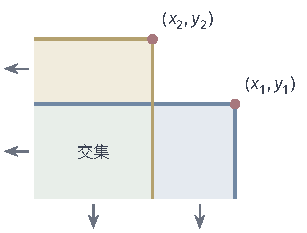
\includegraphics[width=52mm]{figures/07-probability/02-measure-theoretic-probability/tikz/pspace-pi-system/figure.pdf}
  \caption{左下象限构成$\pi$系统。以$(x_1,y_1)$为顶点的象限（浅蓝，蓝色边界）与以$(x_2,y_2)$为顶点的象限（浅黄，黄色边界）都向左、向下无限延伸，它们的交集（浅绿）仍是左下象限，顶点为$(\min\{x_1,x_2\},\min\{y_1,y_2\})$。}
  \label{fig:pspace-pi-system}
\end{BookInlineFigure}

\paragraph{分组保持独立}
第~\ref{chap:random-vectors}章还使用过一个事实：相互独立的变量分成互不相交的几组，各组的函数仍相互独立，例如$X_1+X_2$与$X_3^{2}$独立。现在可以对一般的可测函数证明它。

\begin{theorem}[分组定理]
\label{thm:pspace-grouping}
设$\{\mathcal{G}_i\}_{i\in I}$相互独立，$I_1,I_2,\dots$是$I$的两两不交的子集。令$\mathcal{H}_k$为由$\bigcup_{i\in I_k}\mathcal{G}_i$生成的$\sigma$代数。则$\mathcal{H}_1,\mathcal{H}_2,\dots$相互独立。
\end{theorem}

\begin{proof}
只需证明任意有限个$\mathcal{H}_1,\dots,\mathcal{H}_m$相互独立。令$\mathcal{C}_k$为形如$A_{i_1}\cap\cdots\cap A_{i_r}$的集合全体，其中$i_1,\dots,i_r$是$I_k$中有限个不同的指标，$A_{i_j}\in\mathcal{G}_{i_j}$。$\mathcal{C}_k$对交封闭，含有$\Omega$，且生成$\mathcal{H}_k$。

取$C_k\in\mathcal{C}_k$，$k=1,\dots,m$。不同组的指标互不相同，$C_1\cap\cdots\cap C_m$是来自有限个不同$\mathcal{G}_i$的事件之交。由$\{\mathcal{G}_i\}$的独立性，它的概率等于所有这些事件的概率之积；把乘积按组归并，又等于$\mathbb{P}(C_1)\cdots\mathbb{P}(C_m)$。由引理~\ref{lem:pspace-pi-independence}，$\mathcal{H}_1,\dots,\mathcal{H}_m$相互独立。
\end{proof}

若$X_1,X_2,X_3$相互独立，取$I_1=\{1,2\}$，$I_2=\{3\}$，则$\sigma(X_1,X_2)$与$\sigma(X_3)$独立。这里用到$\sigma(X_1,X_2)$就是由$\sigma(X_1)\cup\sigma(X_2)$生成的$\sigma$代数，因为$\mathcal{B}(\mathbb{R}^{2})$由矩形$B_1\times B_2$生成，而矩形的原像是
\[
  \{(X_1,X_2)\in B_1\times B_2\}=\{X_1\in B_1\}\cap\{X_2\in B_2\}.
\]
对任意Borel函数$g,h$，由上一节“函数只会减少信息”，$\sigma(g(X_1,X_2))\subseteq\sigma(X_1,X_2)$，$\sigma(h(X_3))\subseteq\sigma(X_3)$，所以$g(X_1,X_2)$与$h(X_3)$独立。$g$、$h$不必连续，也不必使原像是区间。

\paragraph{乘积测度给出独立对}
现在转向构造。给定两个概率空间$(E_1,\mathcal{E}_1,P_1)$与$(E_2,\mathcal{E}_2,P_2)$，要造一对独立的随机对象，分布分别是$P_1$和$P_2$。卷四的乘积测度正好做这件事：在$E_1\times E_2$上，乘积$\sigma$代数$\mathcal{E}_1\otimes\mathcal{E}_2$由可测矩形$A\times B$生成，其上存在唯一的概率测度$P_1\otimes P_2$，使
\begin{equation}
  (P_1\otimes P_2)(A\times B)=P_1(A)\,P_2(B),\qquad A\in\mathcal{E}_1,\ B\in\mathcal{E}_2 .
  \label{eq:pspace-product-measure}
\end{equation}
取$\Omega=E_1\times E_2$与$\mathbb{P}=P_1\otimes P_2$，令$X$、$Y$分别取$\omega=(\omega_1,\omega_2)$的第一、第二个坐标。这时
\[
  \{X\in A\}\cap\{Y\in B\}=A\times B,
\]
式~\eqref{eq:pspace-product-measure}说的正是$X$与$Y$独立，且$P_X=P_1$，$P_Y=P_2$。

反过来，独立性也可以完全用联合分布刻画。

\begin{theorem}[独立与乘积分布]
\label{thm:pspace-independence-product}
设$X,Y$分别取值于$(E_1,\mathcal{E}_1)$与$(E_2,\mathcal{E}_2)$。则$X$与$Y$独立，当且仅当
\begin{equation}
  P_{(X,Y)}=P_X\otimes P_Y .
  \label{eq:pspace-independence-product}
\end{equation}
\end{theorem}

\begin{proof}
若式~\eqref{eq:pspace-independence-product}成立，在矩形上取值就得到$\mathbb{P}(X\in A,Y\in B)=P_X(A)P_Y(B)$，即独立。反过来，若$X,Y$独立，则$P_{(X,Y)}$与$P_X\otimes P_Y$在全部可测矩形上取值相同。可测矩形对交封闭，因为
\[
  (A\times B)\cap(A'\times B')=(A\cap A')\times(B\cap B'),
\]
并且它们生成$\mathcal{E}_1\otimes\mathcal{E}_2$。两个概率测度在生成的$\pi$系统上一致，就处处一致。
\end{proof}

这个定理把“独立”从样本空间上的乘法公式，变成了取值空间上的一句话：联合分布是边缘分布的乘积。有密度时可以进一步写成密度的乘积。设$X,Y$分别有密度$f_X,f_Y$。由Tonelli定理，对矩形，
\[
  (P_X\otimes P_Y)(A\times B)=\int_Af_X\,\mathrm{d}x\int_Bf_Y\,\mathrm{d}y=\iint_{A\times B}f_X(x)f_Y(y)\,\mathrm{d}x\,\mathrm{d}y,
\]
再用$\pi$系统论证推广到一切Borel集，所以$f_X(x)f_Y(y)$是$P_X\otimes P_Y$的密度。于是：$X$与$Y$独立，当且仅当$f_X(x)f_Y(y)$是$(X,Y)$的一个联合密度。若$(X,Y)$另有联合密度$f$，同一个测度的两个密度只能在Lebesgue测度为零的集合上不同，可参考\BookChapterRef{chap:measure-densities}{卷四第8章“测度的密度”}；所以独立等价于$f=f_Xf_Y$几乎处处成立。这正是第~\ref{chap:random-vectors}章提到的情形：把联合密度在一条直线上改掉，它仍是联合密度，独立性不受影响。

\paragraph{一个独立对的计算}
设$X\sim\operatorname{Unif}(0,1)$，$Y\sim\operatorname{Exp}(1)$，二者独立，即$(X,Y)$的分布是$\operatorname{Unif}(0,1)\otimes\operatorname{Exp}(1)$。矩形事件直接相乘：
\[
  \mathbb{P}\bigl(X\leq\tfrac12,\ Y>1\bigr)=\tfrac12\cdot\mathrm{e}^{-1}\approx0.1839 .
\]
非矩形事件要对乘积测度积分。事件$\{Y>X\}$是正方形上方、对角线以上的区域。按$x$切片，每条竖直切片$\{y>x\}$在$Y$的分布下的质量是$\mathrm{e}^{-x}$，再对$x$在均匀分布下积分：
\[
  \mathbb{P}(Y>X)=\int_0^1\mathbb{P}(Y>x)\,\mathrm{d}x=\int_0^1\mathrm{e}^{-x}\,\mathrm{d}x=1-\mathrm{e}^{-1}\approx0.6321 .
\]
图~\ref{fig:pspace-product-measure}画出了这两个事件。第二步按切片积分的依据是Tonelli定理：被积函数是区域的示性函数，非负，可以先对$y$积分再对$x$积分。

\begin{BookInlineFigure}
  \centering
  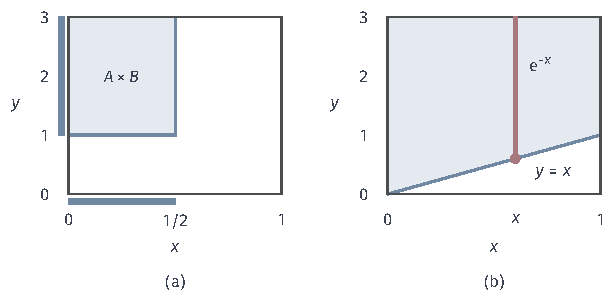
\includegraphics[width=104mm]{figures/07-probability/02-measure-theoretic-probability/tikz/pspace-product-measure/figure.pdf}
  \caption{$\operatorname{Unif}(0,1)\otimes\operatorname{Exp}(1)$上的两个事件，纵轴只画到$y=3$，区域向上延伸。(a)矩形$A\times B$，$A=[0,\tfrac12]$，$B=(1,\infty)$（坐标轴旁的粗线段），概率是两段边缘概率之积；(b)区域$\{y>x\}$，红色竖线是$x$处的切片，它在$Y$的分布下的质量是$\mathrm{e}^{-x}$。}
  \label{fig:pspace-product-measure}
\end{BookInlineFigure}

\paragraph{无穷多次抛硬币}
有限个独立对象由有限次乘积得到，可数个则需要无穷乘积。对实值的情形，木棍上的一个均匀点已经足够。仍取$\Omega=[0,1)$、长度测度，以及上一节的二进制数字$D_k(\omega)$。

\begin{theorem}[二进制数字独立]
\label{thm:pspace-binary-digits}
在$([0,1),\mathcal{B}([0,1)),\lambda)$上，$D_1,D_2,\dots$相互独立，且都服从$\operatorname{Bern}(1/2)$。
\end{theorem}

\begin{proof}
固定$n$与$d_1,\dots,d_n\in\{0,1\}$，令$a=\sum_{k=1}^{n}d_k2^{-k}$。按$D_k$的定义，$\omega$的前$n$位数字依次是$d_1,\dots,d_n$，当且仅当$\lfloor2^{n}\omega\rfloor=2^{n}a$，即
\[
  \{D_1=d_1,\dots,D_n=d_n\}=\bigl[a,\ a+2^{-n}\bigr).
\]
这个区间的长度是$2^{-n}$，所以
\[
  \mathbb{P}(D_1=d_1,\dots,D_n=d_n)=2^{-n}.
\]

对单个数字，把前$n$位中其余$n-1$位的所有取值加起来，得$\mathbb{P}(D_k=d)=2^{n-1}\cdot2^{-n}=1/2$。于是对前$n$个数字，联合概率等于各自概率之积。任意有限个数字都包含在某个前$n$个之中，对不出现的数字求和即可，所以任意有限子族满足乘法公式。数字只取两个值，$\sigma(D_k)$由$\{D_k=1\}$生成，乘法公式对$\sigma(D_k)$中的四个事件都成立。
\end{proof}

图~\ref{fig:pspace-binary-digits}画出了前三位数字。事件$\{D_1=1,D_3=0\}$由两段长$1/8$的区间组成，总长度$1/4=\frac12\cdot\frac12$，与乘法公式一致。

\begin{BookInlineFigure}
  \centering
  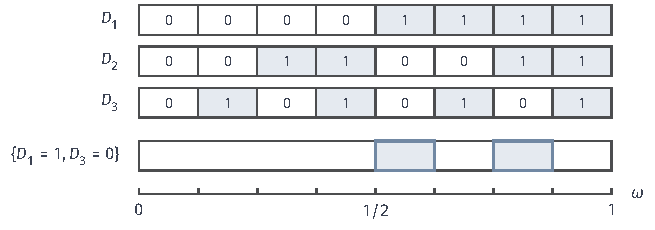
\includegraphics[width=111mm]{figures/07-probability/02-measure-theoretic-probability/tikz/pspace-binary-digits/figure.pdf}
  \caption{$[0,1)$上的二进制数字。前三行中，每个长$1/8$的格子里写着其中各点的第$k$位数字，浅蓝格子取值为$1$。最下一行是事件$\{D_1=1,D_3=0\}=[\tfrac12,\tfrac58)\cup[\tfrac34,\tfrac78)$，长度$\tfrac14$。}
  \label{fig:pspace-binary-digits}
\end{BookInlineFigure}

于是“无穷多次独立抛公平硬币”有了一个具体模型：样本点是木棍上的一个点，第$k$次的结果是它的第$k$位二进制数字。第~\ref{chap:random-variables}章的Cantor变量$\sum_k2D_k/3^{k}$就定义在这个空间上。“首次出现正面的次数”$T=\min\{k:D_k=1\}$也是如此，事件“永远不出现正面”是$\{T=\infty\}=\{0\}$：它非空，概率却为零，是第~\ref{sec:pspace-null-events}节所说的零概率而非不可能事件。

\paragraph{可数个独立的任意分布}
一个均匀点的数字可以拆成可数多组，每组再拼成一个均匀点。正整数$n$可以唯一地写成$n=2^{k-1}(2j-1)$，其中$k,j\geq1$：$k-1$是$n$中因子$2$的个数，$2j-1$是剩下的奇数部分。于是位置集合
\[
  I_k=\{2^{k-1}(2j-1):\ j=1,2,\dots\},\qquad k=1,2,\dots
\]
两两不交，并且覆盖全部正整数。令
\begin{equation}
  U_k=\sum_{j=1}^{\infty}D_{2^{k-1}(2j-1)}\,2^{-j},
  \label{eq:pspace-digit-split}
\end{equation}
即用第$k$组数字依次作为$U_k$的二进制数字（图~\ref{fig:pspace-digit-interleave}）。

\begin{BookInlineFigure}
  \centering
  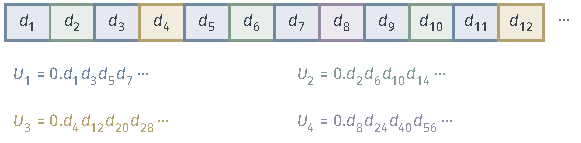
\includegraphics[width=98mm]{figures/07-probability/02-measure-theoretic-probability/tikz/pspace-digit-interleave/figure.pdf}
  \caption{把一个均匀点的二进制数字$d_1d_2d_3\cdots$分成互不相交的组。第$k$组由位置$2^{k-1}(2j-1)$组成，颜色相同的格子属于同一组：奇数位置给$U_1$（蓝），$2,6,10,\dots$给$U_2$（绿），$4,12,20,\dots$给$U_3$（黄），$8,24,\dots$给$U_4$（紫）。}
  \label{fig:pspace-digit-interleave}
\end{BookInlineFigure}

\begin{theorem}[独立序列的存在]
\label{thm:pspace-independent-sequence}
设$F_1,F_2,\dots$是一列满足定理~\ref{thm:pspace-cdf-measure}条件的函数。则在$([0,1),\mathcal{B}([0,1)),\lambda)$上存在相互独立的随机变量$X_1,X_2,\dots$，使$F_{X_k}=F_k$对每个$k$成立。
\end{theorem}

\begin{proof}
分三步。第一步说明$U_1,U_2,\dots$相互独立。$U_k$是第$k$组数字的部分和之极限，可测函数列的极限可测，所以$U_k$关于$\mathcal{H}_k=\sigma(D_n:n\in I_k)$可测，$\sigma(U_k)\subseteq\mathcal{H}_k$。各组位置互不相交，由定理~\ref{thm:pspace-binary-digits}与分组定理~\ref{thm:pspace-grouping}，$\mathcal{H}_1,\mathcal{H}_2,\dots$相互独立，于是$U_1,U_2,\dots$相互独立。

第二步说明每个$U_k$都是均匀分布。$U_k$的数字序列与$(D_1,D_2,\dots)$同样是独立的公平比特。对二进分点区间$J=[b2^{-m},(b+1)2^{-m})$，$U_k\in J$意味着$U_k$的前$m$位数字是$b$的二进制表示，除非$U_k$的数字从某一位起全为$1$。后一情形的概率为零：对固定的起始位置，“此后$r$位全为$1$”的概率是$2^{-r}$，令$r\to\infty$得零，再对可数个起始位置取并。于是
\[
  \mathbb{P}(U_k\in J)=2^{-m}=\lambda(J).
\]
二进分点区间与空集一起构成$\pi$系统，生成$\mathcal{B}([0,1))$，并且$\mathbb{P}(U_k\in[0,1))=1$，所以$U_k$的分布就是长度测度。

第三步作分位数变换。令$Q_k$为$F_k$的分位数函数，$U_k\in(0,1)$时令$X_k=Q_k(U_k)$，否则令$X_k=0$。$U_k$均匀分布，由定理~\ref{thm:pspace-quantile-transform}的证明，$F_{X_k}=F_k$。每个$X_k$是$U_k$的函数，由分组定理，$X_1,X_2,\dots$相互独立。
\end{proof}

第一部分及后续各章常说“取独立同分布的$X_1,X_2,\dots$”，这个定理保证了这样的序列确实存在，而且可以放在同一个概率空间上。取值于$\mathbb{R}^{d}$时，把每个$U_k$的数字再拆成$d$组，就得到$d$个独立坐标。对任意一列概率空间$(E_k,\mathcal{E}_k,P_k)$，可数乘积$\bigotimes_kP_k$在由“只限制有限个坐标”的柱集生成的$\sigma$代数上也存在且唯一，这一般性结论需要测度延拓的进一步论证，篇幅较长，读者可查阅~\scite{math-kallenberg2021probability}。本卷用到的独立序列都是实值或向量值的，上面的构造已经够用。

指标不可数时情况不同。连续时间的随机过程$\{X_t\}_{t\geq0}$也可以按有限个时刻的联合分布在乘积空间上构造，但“路径连续”这样的性质涉及不可数个时刻，不是由有限个坐标决定的事件，第~\ref{sec:pspace-null-events}节的尖峰例子已经显示了这类困难。处理它需要选择合适的版本并证明路径的正则性，可参考\BookChapterRef{chap:stochastic-processes-and-information}{卷九第2章“随机过程与随时间增长的信息”}。
